\section{Experiments}

\subsection{Sweep 1 — Protocol $\times$ Topology}
We hold $N_{\text{agents}} = 3$ and \texttt{task\_type} = \textsc{code} and
run the full $3 \times 3$ factorial design at $T = 0.7$. Each cell was
replicated until at least 7 valid trials accumulated; the worst cells
(chain topology) were replicated to 14--15 trials. After replication the
sweep contains 105 trials in total (some valid, some rate-limit crashes;
crashes are conservatively counted as FC2 failures since the inter-agent
flow broke). Table~\ref{tab:sweep1} reports per-cell FC2 means and
Figure~\ref{fig:fc2_heatmap} visualises them as a heatmap.

\begin{table}[h]
\centering
\caption{Sweep~1 FC2 rates by cell (105 trials at $T=0.7$, $N=3$, code).
Lower is better. Cell counts are valid trials.}
\label{tab:sweep1}
\begin{tabular}{llcc}
\toprule
Protocol & Topology & FC2 & $n$ \\
\midrule
\textsc{a2a}    & \textsc{centralized}      & \textbf{0.07} & 15 \\
\textsc{a2a}    & \textsc{chain}            & 0.30 & 10 \\
\textsc{a2a}    & \textsc{fully\_connected} & 0.30 & 10 \\
\textsc{mcp}    & \textsc{centralized}      & 0.20 & 10 \\
\textsc{mcp}    & \textsc{chain}            & 0.47 & 15 \\
\textsc{mcp}    & \textsc{fully\_connected} & 0.30 & 10 \\
\textsc{native} & \textsc{centralized}      & 0.20 & 10 \\
\textsc{native} & \textsc{chain}            & 0.53 & 15 \\
\textsc{native} & \textsc{fully\_connected} & 0.10 & 10 \\
\bottomrule
\end{tabular}
\end{table}

\begin{figure}[h]
\centering
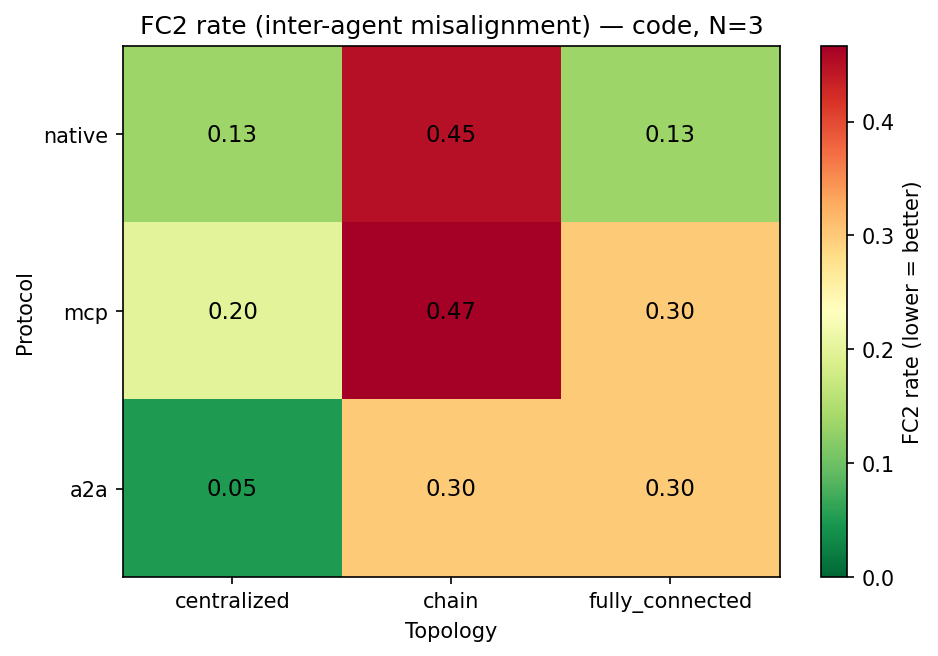
\includegraphics[width=0.7\linewidth]{../figures/fig1_fc2_heatmap.png}
\caption{FC2 rate across the protocol $\times$ topology grid.}
\label{fig:fc2_heatmap}
\end{figure}

\paragraph{ANOVA.} A trial-level one-way ANOVA on FC2 reveals a
significant main effect of \emph{topology} ($F(2,102) = 4.44$,
$p = 0.014$); the main effect of \emph{protocol} does not reach
significance ($F(2,102) = 0.89$, $p = 0.42$). A two-way ANOVA confirms
this dissociation: topology $p = 0.025$, protocol $p = 0.65$,
interaction $p = 0.63$. Welch's $t$-test contrasting the best cell
(\textsc{a2a} $\times$ \textsc{centralized}) against the worst
(\textsc{native} $\times$ \textsc{chain}) is significant: $t = -2.62$,
$p = 0.017$. FC1 and FC3 show no protocol or topology effect
(all $p > 0.40$).

\subsection{Sweep 2 — Agent count}
For \textsc{a2a} $\times$ \textsc{centralized} we vary
$N_{\text{agents}} \in \{2, 3, 4, 5\}$. FC2 increases monotonically with
$N$: 0.0 / 0.0 / 0.2 / 0.4. Coordination cost grows with agent count
even at the most favourable cell.

\subsection{Sweep 3 — Task generality}
Holding the best cell (\textsc{a2a} $\times$ \textsc{centralized},
$N{=}3$) we vary \texttt{task\_type} $\in \{\textsc{code}, \textsc{qa},
\textsc{planning}\}$. FC2 is preserved on \textsc{qa} (0.0) but
catastrophically degrades on \textsc{planning} (1.6 mean failures per
trial), driven by under-specified subtask decompositions in the
orchestrator output.

\subsection{Temperature ablation}
We re-ran the entire $3 \times 3$ grid at $T = 0.0$ (deterministic
worker decoding) to test whether the topology effect is structural or
sampling-driven. \emph{Eight of nine cells collapse to FC2 = 0} on valid
trials. The single exception is \textsc{mcp} $\times$
\textsc{centralized}, which retains FC2 = 0.25 across 8 valid trials
pooled over four independent re-runs. Trace inspection shows the
orchestrator wraps its own integration step in
\texttt{<mcp:message>} envelopes addressed back to itself, and
executors parse only a partial envelope and act on the misread. This
is a structural failure of the protocol, not amplified sampling
variance, and is the cleanest reproducible MAST-FC2 trigger we
identify.

\begin{figure}[h]
\centering
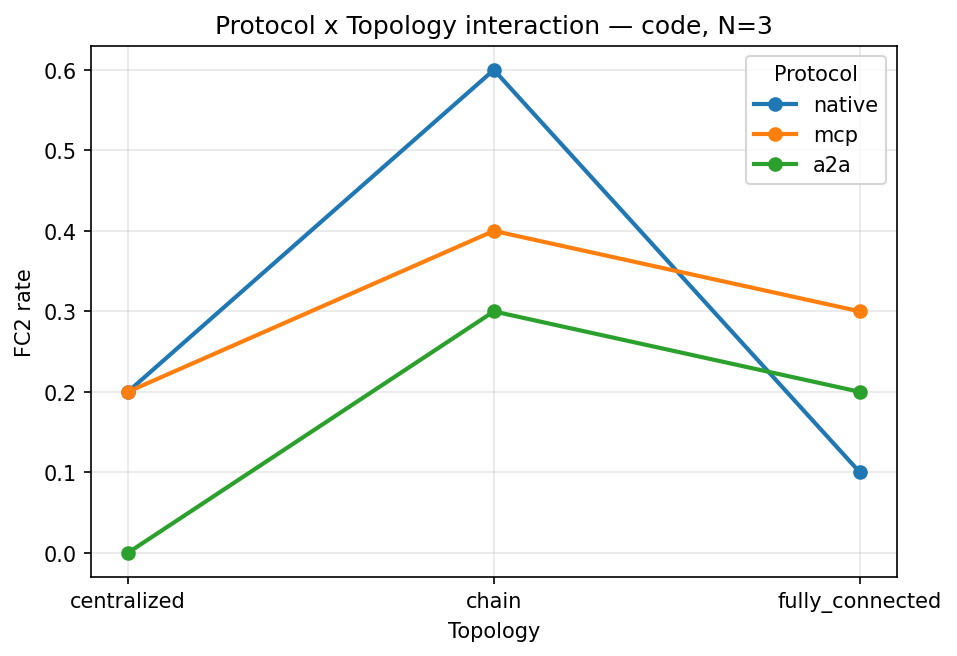
\includegraphics[width=0.7\linewidth]{../figures/fig3_interaction.png}
\caption{Protocol $\times$ topology interaction plot for FC2 rate at
$T=0.7$. The chain topology penalty is largest for \textsc{native} and
\textsc{mcp}; centralized rescues all three protocols.}
\label{fig:interaction}
\end{figure}

\paragraph{Reframing.} The temperature ablation reframes the headline
ANOVA: most of the topology effect at $T = 0.7$ is sampling-variance
amplification (chain topologies have less cross-stage visibility, so
sampling noise propagates farther), \emph{not} a structural coordination
property. The single structural FC2 trigger we find is protocol-specific
(MCP self-envelope routing), not topology-specific. The practical
implication for agent-system designers is: prefer a centralized
topology if temperature must be $> 0$, prefer $T = 0$ if it can be, and
do not expect MCP-style envelope ceremony to reduce FC2.
